\section{A Synthetic Where's-Waldo Benchmark}
\label{sec:benchmark}

\begin{figure}[t]
  \centering
  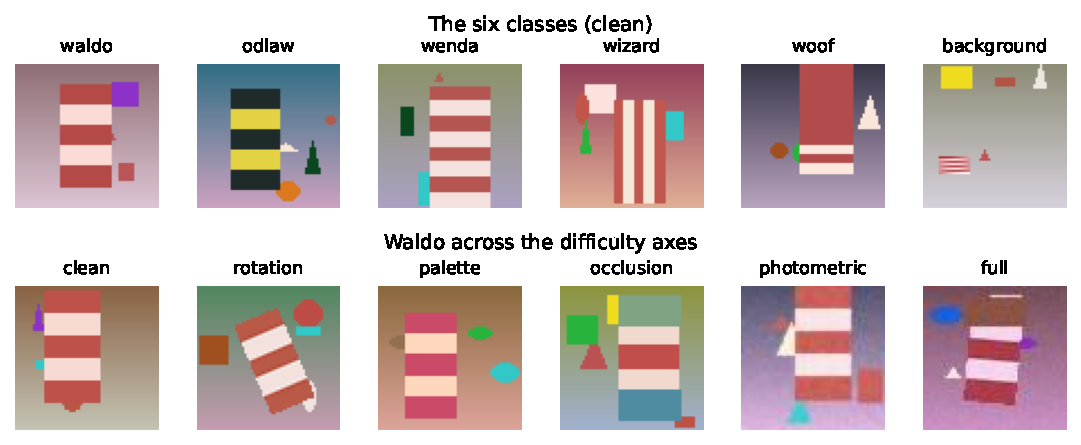
\includegraphics[width=0.98\textwidth]{figures/classes_difficulty.pdf}
  \caption{The synthetic benchmark. Top: one clean patch of each of the six classes---the target Waldo and four look-alikes that each differ from him on a single feature (Odlaw's palette, Wenda's stripe count, Wizard's orientation, Woof's partial band), plus a background class of distractors and striped clutter. Bottom: the same Waldo under each difficulty axis (rotation, palette jitter, occlusion, photometric degradation) and all of them combined.}
  \label{fig:classes}
\end{figure}

Where's Waldo is a recognizable visual-search puzzle in which the reader must find one unremarkable figure among hundreds, aided and hindered by a recurring cast of look-alikes (Odlaw, Wenda, Wizard Whitebeard, and the dog Woof) that the artist draws to resemble Waldo. That built-in cast of near-duplicates makes the puzzle a convenient testbed for a recognizer, and machine-learning treatments of it exist~\cite{barthelmes2021wally}. We use a synthetic version rather than the books because the experiments need controlled material the published pages cannot give: many balanced instances of each character, difficulty we can vary, and a known target location in every scene. The largest annotated real collection, Hey-Waldo~\cite{constantinou2017heywaldo}, marks the target in only 14 scenes at one instance per page, which is enough to calibrate against but not to run an experiment on, so we measure those pages and match the generator to them: Waldo's red is a muted (185, 84, 78) and his white a cream (247, 225, 217), his width a median 1.4\% of the page at aspect 0.52, with red covering roughly 17\% of the whole page and white 22\%. Because the page is as red-and-white as Waldo himself, colour alone cannot locate him, so the benchmark inherits a task that rewards stripe structure over palette.

The generator abstracts each character to the one structural trait that survives a small patch. In the books the characters are told apart by fine facial detail, which is lost once a figure shrinks to the few-dozen pixels a recognizer sees, so we keep instead the trait that does survive: a character's palette, stripe orientation, stripe layout, or completeness. This gives six classes (Figure~\ref{fig:classes}): the target Waldo and four look-alikes (Odlaw in a black-and-yellow palette, Wenda with a different stripe count, Wizard with vertical stripes, and Woof showing only a partial striped band), plus a background class. Each look-alike differs from Waldo on exactly one feature, which makes it a controlled hard negative, and the background class is not blank canvas but distractors and striped clutter (barber poles, awnings, flags) that share Waldo's colour and stripe texture while differing in scale and shape, so a model cannot succeed by flagging any red-and-white stripe.

From this shared machinery the generator emits two products. For recognition it draws balanced 48$\times$48 patches, one character or none per patch, which the encoding study and the unlearning experiments consume. For localization it composes cluttered scenes with one Waldo at a known position among friends and clutter, returning that position as the label against which the sliding-window localizer of Section~\ref{sec:encoding} is scored. Both products share four difficulty axes (rotation, palette jitter, occlusion, and a photometric degradation that mimics a photographed page) applied one at a time or together, so every comparison runs from clean to severe and difficulty is set to be hard for all models rather than tuned against one.

A reduced task would be worthless if a simple rule could read the class off each patch, so we check. A depth-three decision tree over aggregate colour and stripe statistics reaches only about 0.5 macro-F1 on clean patches, while the same patches let a model trained on raw pixels reach about 0.95, and the gap holds as difficulty rises, because the distinguishing traits (how many stripes, where the band sits, how the pattern is arranged) live in a spatial layout that aggregate statistics discard. We release the generator openly, so the benchmark is reproducible from a seed. Because the same identities recur in controlled volume, this generator supplies both the recognition workloads that the unlearning study deletes from in Section~\ref{sec:unlearning} and the scenes that the localizer reads in Section~\ref{sec:encoding}.
